\chapter{図形埋め込みのサンプル}
\label{sec:figure_sample}

この章では各種形式の図形を埋め込む例を示します。

\section{PDF図形の埋め込み}
\begin{wrapfigure}[9]{O}[0pt]{0\textwidth}
  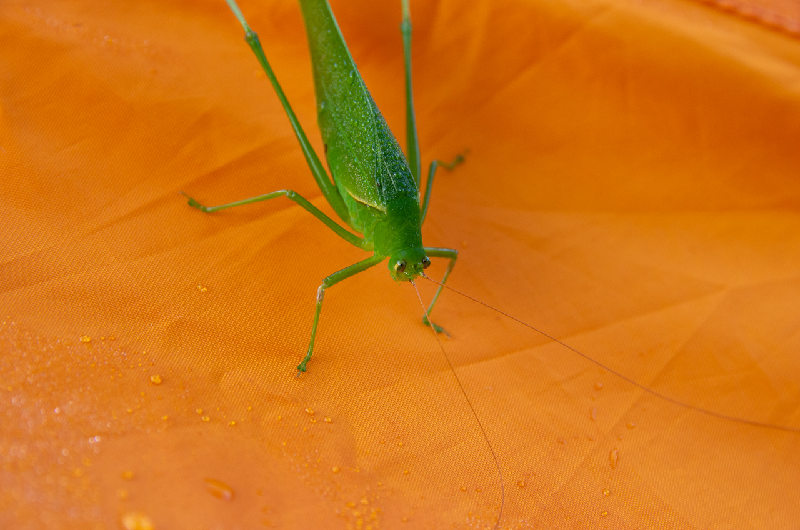
\includegraphics[width=5cm,pagebox=cropbox,clip]{image/IMGP3933.pdf}
  \caption{PDF図形の埋め込み}\label{embeded_pdf}
\end{wrapfigure}

プロジェクト内部のimage\_srcディレクトリに置かれたPDFファイルは\LaTeX\
処理直前にimageディレクトリにそのままコピーされます。この際、
処理の対象になるのは拡張子が"pdf"であるようなファイルのみです。
Unixファイルシステムは大文字と小文字を区別することに注意してください。
拡張子"PDF"は無視されます。

したがって、\LaTeX\ 文書内部ではimage/filename.pdfとして参照することで
文書内にPDF図形を表示できます。

\section{JPEG図形の埋め込み}

\begin{wrapfigure}[9]{O}[0pt]{0\textwidth}
  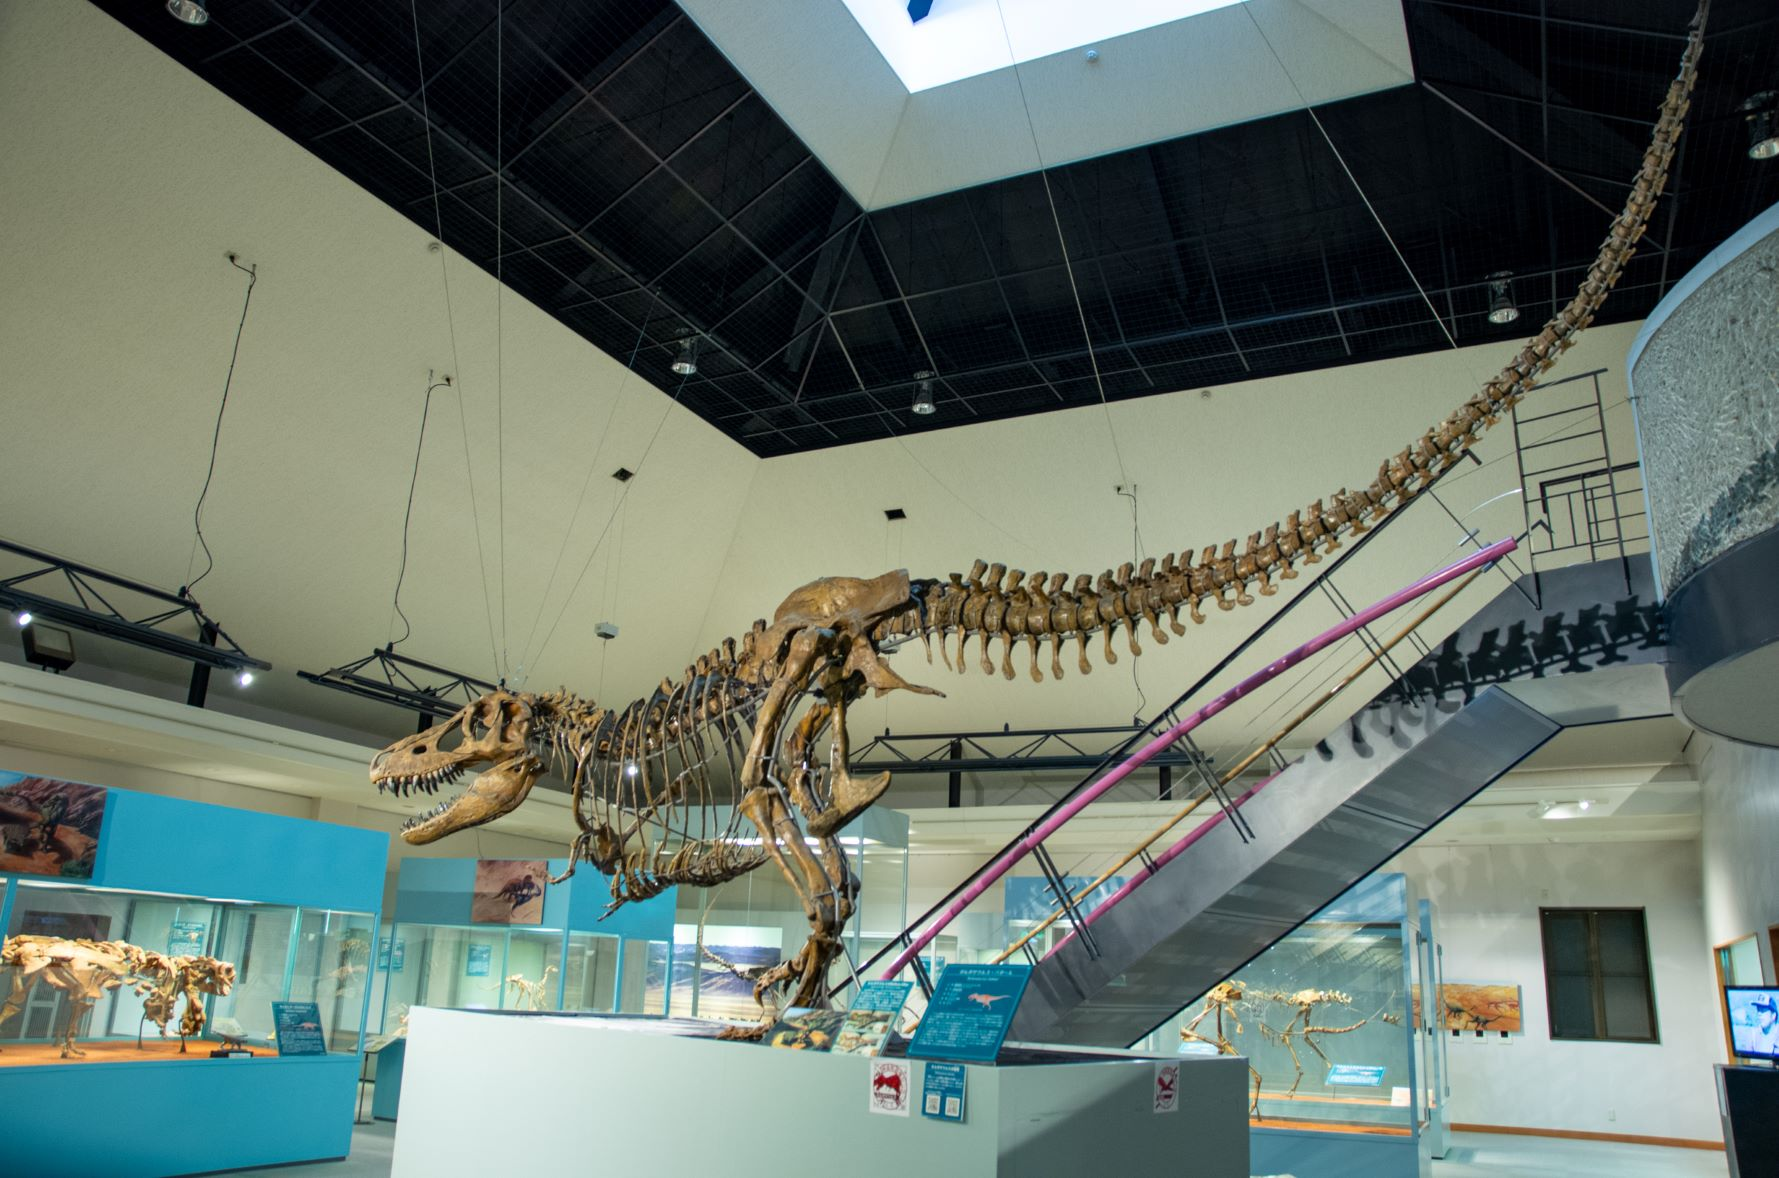
\includegraphics[width=5cm,pagebox=cropbox,clip]{image/IMGP3954.pdf}
  \caption{JPEG図形の埋め込み}\label{embeded_jpeg}
\end{wrapfigure}

同様にプロジェクト内部のimage\_srcディレクトリに置かれたJPEGファイルは\LaTeX\
処理直前にPDFファイルに変換されてimageディレクトリにコピーされます。この際、
処理の対象になるのは拡張子が"jpg"であるようなファイルのみです。
Unixファイルシステムは大文字と小文字を区別することに注意してください。
拡張子"JPG"は無視されます。

したがって、\LaTeX\ 文書内部ではimage/filename.pdfとして参照することで
文書内にPDF図形を表示できます。

埋め立て文字。埋め立て文字。埋め立て文字。埋め立て文字。
埋め立て文字。埋め立て文字。埋め立て文字。埋め立て文字。
埋め立て文字。埋め立て文字。埋め立て文字。埋め立て文字。
埋め立て文字。埋め立て文字。埋め立て文字。埋め立て文字。
埋め立て文字。埋め立て文字。埋め立て文字。埋め立て文字。
埋め立て文字。埋め立て文字。埋め立て文字。埋め立て文字。
埋め立て文字。埋め立て文字。埋め立て文字。埋め立て文字。

\section{PNG図形の埋め込み}

\begin{wrapfigure}[10]{O}[0pt]{0\textwidth}
  
\includegraphics[width=5cm,pagebox=cropbox,clip]{image/paint1.pdf}
  \caption{PNG図形の埋め込み}\label{embeded_png}
\end{wrapfigure}

また、image\_srcディレクトリに置かれたPNGファイルは\LaTeX\
処理直前にPDFファイルに変換されてimageディレクトリにコピーされます。この際、
処理の対象になるのは拡張子が"png"であるようなファイルのみです。
Unixファイルシステムは大文字と小文字を区別することに注意してください。
拡張子"PNG"は無視されます。

したがって、\LaTeX\ 文書内部ではimage/filename.pdfとして参照することで
文書内にPDF図形を表示できます。

\section{GIF図形の埋め込み}

\begin{wrapfigure}[10]{O}[0pt]{0\textwidth}
  \includegraphics[width=5cm,pagebox=cropbox,clip]{image/paint2.pdf}
  \caption{GIF図形の埋め込み}\label{embeded_gif}
\end{wrapfigure}

さらに、image\_srcディレクトリに置かれたGIFファイルは\LaTeX\
処理直前にPDFファイルに変換されてimageディレクトリにコピーされます。この際、
処理の対象になるのは拡張子が"gif"であるようなファイルのみです。
Unixファイルシステムは大文字と小文字を区別することに注意してください。
拡張子"GIF"は無視されます。

埋め立て文字。埋め立て文字。埋め立て文字。埋め立て文字。
埋め立て文字。埋め立て文字。埋め立て文字。埋め立て文字。
埋め立て文字。埋め立て文字。埋め立て文字。埋め立て文字。

埋め立て文字。埋め立て文字。埋め立て文字。埋め立て文字。
埋め立て文字。埋め立て文字。埋め立て文字。埋め立て文字。
埋め立て文字。埋め立て文字。埋め立て文字。埋め立て文字。
埋め立て文字。埋め立て文字。埋め立て文字。埋め立て文字。
埋め立て文字。埋め立て文字。埋め立て文字。埋め立て文字。
埋め立て文字。埋め立て文字。埋め立て文字。埋め立て文字。
埋め立て文字。埋め立て文字。埋め立て文字。埋め立て文字。


\section{DRAWIO図形の埋め込み}

\begin{wrapfigure}[10]{O}[0pt]{0\textwidth}
  \includegraphics[width=3cm,pagebox=cropbox,clip]{image/diagram.pdf}
  \caption{DRAWIO図形の埋め込み}\label{embeded_drawio}
\end{wrapfigure}

さらに、image\_srcディレクトリに置かれた\term{DRAWIO}ファイルは\LaTeX\
処理直前にPDFファイルに変換されてimageディレクトリにコピーされます。

この際、
処理の対象になるのは拡張子が"drawio"であるようなファイルのみです。
Unixファイルシステムは大文字と小文字を区別することに注意してください。
拡張子"DRAWIO"は無視されます。

